\documentclass[11pt]{article}
\usepackage{header_problems}
\usepackage{header_template}
\usepackage{txfonts}
\usepackage{enumitem}
\def\title{HW3}

\begin{document}
\maketitle
\fontsize{12}{15}\selectfont


%\excludecomment{solution}

\textbf{Due: Wednesday, February 23 at 11:59 pm}
\newline

This homework consists of coding assignments and math problems. \\
\textbf{Begin early; you can submit models to Kaggle only twice a day!}

\textbf{DELIVERABLES:}

\begin{enumerate}[topsep=1pt]
  \item
    Submit your predictions for the test sets to Kaggle as early as possible. Include your Kaggle scores in your write-up.
    The Kaggle competition for this assignment can be found at
    \begin{itemize}
     \item MNIST: https://www.kaggle.com/c/hw3-mnist-competition-cs189sp22
     \item SPAM: https://www.kaggle.com/c/hw3-spam-competition-cs189sp22
     \end{itemize}

\item \underline{Write-up}: Submit your solution in {\bf PDF} format to
%	the Gradescope assignment entitled 
		``Homework 3 Write-Up'' in Gradescope.
%		Instructions for the write-up:
	\begin{itemize}[topsep=0pt, noitemsep]    
		\item On the first page of your write-up, please list students with whom you collaborated

		\item Start each question on a new
        page. If there are graphs, include those graphs on the same pages as the question write-up. DO NOT put them in an appendix. We need each solution to be self-contained on pages of its own.

		\item \textbf{Only PDF uploads to Gradescope will be accepted}. You are encouraged
			use \LaTeX\ or Word to typeset your solution. You may also scan a neatly handwritten
			solution to produce the PDF. 

		\item \textbf{Replicate all your code in an appendix}. 
			Begin code for each coding question in a fresh page.
			Do not put code from multiple questions in the same page.
			When you upload this PDF on Gradescope, \emph{make sure}
			that you assign the relevant pages of your code from appendix to correct questions.

		\item While collaboration is encouraged, \emph{everything} in your solution must
			be your (and only your) creation. Copying the answers or code of another student is strictly forbidden. Furthermore, all external material 
			(i.e., \emph{anything} outside lectures and assigned
			readings, including figures and pictures) should be cited properly.
			We wish to remind you that consequences of academic misconduct are
			\emph{particularly severe}!
	\end{itemize}

\item \underline{Code}: Submit your code as a .zip file 
	%needed to reproduce your results to the Gradescope assignment entitled 
	to ``Homework 3 Code''.
	\begin{itemize}[topsep=0pt, noitemsep]    
		\item \textbf{Set a seed for all pseudo-random numbers generated in your code.}
			This ensures your results are replicated when readers run your code.
		\item Include a README with your name, student ID,
			the values of random seed (above) you used, and any instructions
			for compilation.
		\item Do NOT provide any data files. Supply instructions on how to
			add data to your code.
		\item Code requiring exorbitant memory or execution time might not be considered.
		\item Code submitted here must match that in the PDF Write-up. The Kaggle score will not be accepted if the code provided a) does not compile or b) compiles
but does not produce the file submitted to Kaggle.
	\end{itemize}
	
	 \item The assignment covers concepts on Gaussian distributions and classifiers. Some of the material may not have been covered in lecture; you are responsible for finding resources to understand it.
\end{enumerate}



% \input{template/getting_started.tex}
\Question{Honor Code}

Declare and sign the following statement (Mac Preview, PDF Expert, and FoxIt PDF Reader, among others, have tools to
let you sign a PDF file): 

\textit{``I certify that all solutions 
are entirely my own and that I have not looked at anyone else's solution. I have given credit to all external sources I consulted."}

Signature: \hrulefill


\Question{Gaussian Classification}


Let $f(x \mid C_i) \sim \mathcal{N}(\mu_i,\sigma^2)$ for
a two-class, one-dimensional classification problem with
classes $C_{1}$ and $C_{2}$,
$P(C_1)=P(C_2)=1/2$, and $\mu_{2} > \mu_{1}$.
\begin{enumerate}
\item
Find the Bayes optimal decision boundary and the corresponding Bayes decision rule by finding the point(s) at which the posterior probabilities are equal.
Use the 0-1 loss function.
\begin{solution}
Your 2.1 solution here
\end{solution}

\item
Suppose the decision boundary for your classifier is $x = b$. The Bayes error is the probability of misclassification, namely, 
$$P_{e} = P((C_1 \text{ misclassified as } C_2) \cup (C_2 \text{ misclassified as } C_1)).$$
Show that the Bayes error associated with this decision rule, in terms of $b$, is
\begin{equation*}
P_e(b) = \frac{1}{2\sqrt{2\pi}\sigma}\left(\int_{-\infty}^{b} \exp \left(-\frac{(x - \mu_2)^2}{2\sigma^2}\right) \, dx + \int_b^\infty \exp \left(-\frac{(x-\mu_1)^2}{2\sigma^2} \right) \, dx\right).
\end{equation*}
\begin{solution}
Your 2.2 solution here
\end{solution}
\item
Using the expression above for the Bayes error, calculate the optimal decision boundary $b^*$ that minimizes $P_e(b)$. How does this value compare to that found in part 1? \emph{Hint: $P_e(b)$ is convex for $\mu_1 < b < \mu_2$.}

\begin{solution}
Your 2.3 solution here
\end{solution}
\end{enumerate}




\Question{Isocontours of Normal Distributions}

Let $f(\mu,\Sigma)$ be the probability density function of a normally distributed random variable in $\R^2$.
Write code to plot the isocontours of the following functions, each on its own separate figure. Make sure it is clear which figure belongs to which part.
You're free to use any plotting libraries or stats utilities available in your programming language; for instance, in Python you can use Matplotlib and SciPy.
Choose the boundaries of the domain you plot large enough to show the interesting characteristics of the isocontours (use your judgment).
Make sure we can tell what isovalue each contour is associated with---you can do this with labels or a colorbar/legend.

	\begin{enumerate}
		\item $f(\mu,\Sigma)$, where $\mu = \begin{bmatrix} 1 \\ 1\end{bmatrix}$ and $\Sigma = \begin{bmatrix} 1 & 0\\ 0 & 2 \end{bmatrix}$.

		\item $f(\mu,\Sigma)$, where $\mu = \begin{bmatrix} -1 \\ 2\end{bmatrix}$ and $\Sigma = \begin{bmatrix} 2 & 1\\ 1 & 4 \end{bmatrix}$.
		\item $f(\mu_1,\Sigma_1)-f(\mu_2,\Sigma_2)$, where $\mu_1 = \begin{bmatrix} 0 \\ 2\end{bmatrix}$, $\mu_2 = \begin{bmatrix} 2 \\ 0\end{bmatrix}$ and $\Sigma_1 = \Sigma_2 = \begin{bmatrix} 2 & 1\\ 1 & 1 \end{bmatrix}$.
		
		(Yes, this is a difference between two PDFs. No, it is not itself a valid PDF. Just plot its isocontours anyway.)
		\item $f(\mu_1,\Sigma_1)-f(\mu_2,\Sigma_2)$, where $\mu_1 = \begin{bmatrix} 0 \\ 2\end{bmatrix}$, $\mu_2 = \begin{bmatrix} 2 \\ 0\end{bmatrix}$, $\Sigma_1 = \begin{bmatrix} 2 & 1\\ 1 & 1 \end{bmatrix}$ and $\Sigma_2 = \begin{bmatrix} 2 & 1\\ 1 & 4 \end{bmatrix}$.
		\item $f(\mu_1,\Sigma_1)-f(\mu_2,\Sigma_2)$, where $\mu_1 = \begin{bmatrix} 1 \\ 1\end{bmatrix}$, $\mu_2 = \begin{bmatrix} -1 \\ -1\end{bmatrix}$, $\Sigma_1 = \begin{bmatrix} 2 & 0\\ 0 & 1 \end{bmatrix}$ and $\Sigma_2 = \begin{bmatrix} 2 & 1\\ 1 & 2 \end{bmatrix}$.
		
	\begin{solution}
    Your Question 3 solution here: Remember to make a seperate figure for each part and include labels or a legend 
    \end{solution}
	\end{enumerate}

\Question{Eigenvectors of the Gaussian Covariance Matrix}


Consider two one-dimensional random variables $X_1 \sim \mathcal{N}(3,9)$ and $X_2 \sim \frac{1}{2}X_1+\mathcal{N}(4,4)$,  where $\mathcal{N}(\mu, \sigma^2)$ is a Gaussian  distribution with mean $\mu$ and  variance $\sigma^2$.
Write a program that draws $n=100$ random two-dimensional sample points from $(X_1, X_2)$. For each sample point, the value of $X_2$ is a function of the value of $X_1$ for that {\em same} sample point, but the sample points are independent of each other.
In your code, make sure to choose and set a fixed random number seed for whatever random number generator you use, so your simulation is reproducible, and document your choice of random number seed and random number generator in your write-up.
For each of the following parts, include the corresponding output of your program.

\begin{enumerate}
\item
Compute the mean (in $\R^2$) of the sample.

\begin{solution}
Your 4.1 solution here
\end{solution}
\item
Compute the $2 \times 2$ covariance matrix of the sample (based on the sample mean, not the true mean---which you would not know given real-world data).

\begin{solution}
Your 4.2 solution here
\end{solution}

\item
Compute the eigenvectors and eigenvalues of this covariance matrix.

\begin{solution}
Your 4.3 solution here
\end{solution}
\item
On a two-dimensional grid with a horizonal axis for $X_1$ with range $[-15, 15]$ and a vertical axis for $X_2$ with range $[-15, 15]$, plot
\begin{itemize}
	\item[(i)] all $n=100$ data points, and
	\item[(ii)] arrows representing both covariance eigenvectors.  The eigenvector arrows should originate at the mean and have magnitudes equal to their corresponding eigenvalues.
\end{itemize}
Hint:  make {\em sure} your plotting software is set so the figure is square (i.e., the horizontal and vertical scales are the same). Not doing that is the key to hours of frustration!

\begin{solution}
Your 4.4 solution here
\end{solution}
\item
Let $U = [v_1~~~v_2]$ be a $2 \times 2$ matrix whose columns are the {\bf unit} eigenvectors of the covariance matrix, where $v_1$ is the eigenvector with the larger eigenvalue.  We use $U^\top$ as a rotation matrix to rotate each sample point from the $(X_1, X_2)$ coordinate system to a coordinate system aligned with the eigenvectors.  (As $U^\top = U^{-1}$, the matrix $U$ reverses this rotation, moving back from the eigenvector coordinate system to the original coordinate system).  {\em Center} your sample points by subtracting the mean $\mu$ from each point; then rotate each point by $U^\top$, giving $x_{\mathrm{rotated}}=U^\top(x - \mu)$.  Plot these rotated points on a new two dimensional-grid, again with both axes having range $[-15, 15]$.
(You are not required to plot the eigenvectors, which would be horizontal and vertical.)

\begin{solution}
Your 4.5 solution here
\end{solution}
\end{enumerate}

In your plots, {\bf clearly label the axes and include a title}. Moreover, {\bf make sure the horizontal and vertical axis have the same scale!} The aspect ratio should be one.

\newpage
\Question{Classification and Risk}

Suppose we have a classification problem with classes labeled $1, \dotsc, c$ and
an additional ``doubt'' category labeled $c+1$. Let $r : \mathbb{R}^d \to \{1, \dots, c+1 \}$ be a decision rule. Define the loss function
\[
L(r(x) = i, y = j) =
  \begin{cases}
   0 &  \mathrm{if}\ i=j \quad i,j\in\{1,\dotsc,c\}, \\
   \lambda_r       & \mathrm{if}\ i=c+1, \\
   \lambda_s       & \text{otherwise},
  \end{cases}
\]
where $\lambda_r \geq 0$ is the loss incurred for choosing doubt,
$\lambda_s \geq 0$ is the loss incurred for making a misclassification, and at least one of them is nonzero.
Hence the risk of classifying a new data point $x$ as class $i\in\{1,2,\dots,c+1\}$ is
$$R(r(x)=i|x) = \sum_{j=1}^{c} L(r(x) = i, y = j) \, P(Y = j|x).$$
To be clear, the actual label $Y$ can {\em never} be $c + 1$.

\begin{enumerate}
\item Show that the following predictor obtains the minimum risk when $\lambda_r \leq \lambda_s$:
  \begin{itemize}
  \item Choose class~$i$ if $P(Y = i|x) \geq P(Y = j|x)$ for all $j$ and
    $P(Y = i|x) \geq 1-\lambda_r/\lambda_s$;
    \item Choose doubt otherwise.
  \end{itemize}
  
\begin{solution}
Your 5.1 solution here
\end{solution}
\item What happens if $\lambda_r=0$?  What happens if $\lambda_r>\lambda_s$?
  Explain why this is consistent with what one would expect intuitively.
  
\begin{solution}
Your 5.2 solution here
\end{solution}
\end{enumerate}

\Question{Maximum Likelihood Estimation and Bias}

Let $X_1, \ldots, X_n \in \mathbb{R}$ be
$n$ sample points drawn independently from
univariate normal distributions such that $X_i \sim \mathcal{N}(\mu, \sigma_i^2)$, where
$\sigma_i = \sigma / \sqrt{i}$ for some parameter $\sigma$.
(Every sample point comes from a distribution with a {\bf different variance}.) Note the word ``univariate''; we are working in dimension $d = 1$, and our ``points'' are real numbers.

\begin{enumerate}

\item Derive the maximum likelihood estimates, denoted $\hat{\mu}$ and $\hat{\sigma}$, for the mean $\mu$ and the parameter $\sigma$. (The formulae from class don't apply here, because every point has a different variance.) You may write an expression for $\hat{\sigma}^2$ rather than $\hat{\sigma}$ if you wish---it's probably simpler that way.  Show all your work.

\begin{solution}
Your 6.1 solution here
\end{solution}
\item Given the true value of a statistic $\theta$ and an estimator $\hat{\theta}$ of that statistic, we define the \textit{bias} of the estimator to be the the expected difference from the true value. That is,
$$bias(\hat{\theta}) = \mathbb{E}[\hat{\theta}] - \theta.$$
We say that an estimator is \textit{unbiased} if its bias is $0$.

Either prove or disprove the following statement: \textit{The MLE sample estimator $\hat{\mu}$ is unbiased}.
% If you choose to disprove the statement, suggest an alternative estimator, $\tilde{\mu}$ and show that it is unbiased.
\emph{Hint: Neither the true $\mu$ nor true $\sigma^2$ are known when estimating sample statistics, thus we need to plug in appropriate estimators.}

\begin{solution}
Your 6.2 solution here
\end{solution}
\item
Either prove or disprove the following statement: \textit{The MLE sample estimator $\hat{\sigma^2}$ is unbiased}.
% If you choose to disprove the statement, suggest an alternative estimator, $\tilde{\sigma^2}$ and show that it is unbiased.
\emph{Hint: Neither the true $\mu$ nor true $\sigma^2$ are known when estimating sample statistics, thus we need to plug in appropriate estimators.}

\begin{solution}
Your 6.3 solution here
\end{solution}
\end{enumerate}
\Question{Covariance Matrices and Decompositions}

\newcommand{\Var}{\mathrm{Var}}
\newcommand{\Cov}{\mathrm{Cov}}

As described in lecture, the covariance matrix $\Var(R) \in \mathbb{R}^{d \times d}$ for a random variable $R \in \mathbb{R}^d$ with mean $\mu$ is
\[
\Var(R) = \Cov(R, R) = \E[(R - \mu) \, (R - \mu)^\top] =
\left[ \begin{array}{cccc}
\Var(R_1)      & \Cov(R_1, R_2) & \ldots & \Cov(R_1, R_d)  \\
\Cov(R_2, R_1) & \Var(R_2)      &        & \Cov(R_2, R_d)  \\
\vdots         &                & \ddots & \vdots          \\
\Cov(R_d, R_1) & \Cov(R_d, R_2) & \ldots & \Var(R_d)
\end{array} \right],
\]
where $\Cov(R_i, R_j) = \E[(R_i - \mu_i) \, (R_j - \mu_j)]$ and
$\Var(R_i) = \Cov(R_i, R_i)$.

If the random variable $R$ is sampled from the multivariate normal distribution $\mathcal{N}(\mu, \Sigma)$ with the PDF
\[
f(x) = \frac{1}{\sqrt{(2 \pi)^d |\Sigma|}}e^{- ((x - \mu)^\top \Sigma^{-1} (x- \mu)) / 2},
\]
then $\Var(R) = \Sigma$.

Given $n$ points $X_1, X_2, \ldots, X_n$ sampled from $\mathcal{N}(\mu, \Sigma)$, we can estimate $\Sigma$ with the maximum likelihood estimator
\[
\hat{\Sigma} = \frac{1}{n} \sum_{i = 1}^n (X_i - \mu) \, (X_i - \mu)^\top,
\]
which is also known as the covariance matrix of the sample.

\begin{enumerate}
\item
The estimate $\hat{\Sigma}$ makes sense as an approximation of $\Sigma$ only if $\hat{\Sigma}$ is invertible.  Under what circumstances is $\hat{\Sigma}$ not invertible?  Make sure your answer is complete; i.e., it includes all cases in which the covariance matrix of the sample is singular.  Express your answer in terms of the geometric arrangement of the sample points $X_i$.

\begin{solution}
Your 7.1 solution here
\end{solution}
\item
Suggest a way to fix a singular covariance matrix estimator $\hat{\Sigma}$ by replacing it with a similar but invertible matrix.  Your suggestion may be a kludge, but it should not change the covariance matrix too much.  Note that infinitesimal numbers do not exist; if your solution uses a very small number, explain how to calculate a number that is sufficiently small for your purposes.

\begin{solution}
Your 7.2 solution here
\end{solution}
\item
Consider the normal distribution $\mathcal{N}(0, \Sigma)$ with mean $\mu = 0$.  Consider all vectors of length $1$; i.e., any vector $x$ for which $\|x\| = 1$.  Which vector(s) $x$ of length $1$ maximizes the PDF $f(x)$?  Which vector(s) $x$ of length $1$ minimizes $f(x)$?  Your answers should depend on the properties of $\Sigma$.  Explain your answer.

\begin{solution}
Your 7.3 solution here
\end{solution}
\item
Suppose we have $X \sim \mathcal{N}(0, \Sigma)$, $X \in \R^{n}$ and a unit vector $y \in \R^{n}$. We can compute the projection of the random vector $X$ onto a direction $y$ as $p = y^{T} X$. First, compute the variance of $p$. Using this information, describe the statistical significance of the eigenvector corresponding to the largest eigenvalue of the covariance matrix.

\begin{solution}
Your 7.4 solution here
\end{solution}
\end{enumerate}

\newpage
\Question{Gaussian Classifiers for Digits and Spam}

In this problem, you will build classifiers based on Gaussian discriminant analysis. Unlike Homework 1, you are NOT allowed to use any libraries for out-of-the-box classification (e.g. {\tt sklearn}). You may use anything in {\tt numpy} and {\tt scipy}.

The training and test data can be found with this homework. Don't use the training/test data from Homework 1, as they have changed for this homework. You can verify that your data files and python environment are setup properly by running {\tt sanity.py}. Submit your predicted class labels for the test data on the Kaggle competition website and be sure to include your Kaggle display name and scores in your writeup. Also be sure to include an appendix of your code at the end of your writeup.

\begin{enumerate}
\item Taking pixel values as features (no new features yet, please), fit a Gaussian distribution to each digit class using maximum likelihood estimation.  This involves computing a mean and a covariance matrix for each digit class, as discussed in lecture.

\emph{Hint:}  You may, and probably should, contrast-normalize the images before using their pixel values.  One way to normalize is to divide the pixel values of an image by the $l_2$-norm of its pixel values.

\begin{solution}
Your 8.1 solution here
\end{solution}
\item (Written answer + graph)  Visualize the covariance matrix for a particular class (digit).  How do the diagonal terms compare with the off-diagonal terms?  What do you conclude from this?

\begin{solution}
Your 8.2 solution here. Remember to include a graph \textit{and} a written answer.
\end{solution}

\item Classify the digits in the test set on the basis of posterior probabilities with two different approaches. Feel free to either use the starter code provided in {\tt starter.py} or write your own implementation from scratch


\begin{enumerate}
\item (Graphs) Linear discriminant analysis (LDA).  Model the class conditional probabilities as Gaussians $\mathcal{N}(\mu_\mathrm{C}, \Sigma)$ with different means $\mu_\mathrm{C}$ (for class C) and the same pooled within-class covariance matrix $\Sigma$, which you compute from a weighted average of the 10 covariance matrices from the 10 classes, as described in lecture.

In your implementation, you might run into issues of determinants overflowing or underflowing, or normal PDF probabilities underflowing. These problems might be solved by learning about {\tt numpy.linalg.slogdet} and/or {\tt scipy.stats.multivariate\_normal. logpdf}.

  To implement LDA, you will sometimes need to compute a matrix-vector product of the form $\Sigma^{-1} x$ for some vector $x$.  You should {\bf not} compute the inverse of $\Sigma$ (nor the determinant of $\Sigma$) as it is not guaranteed to be invertable. Instead, you should find a way to solve the implied linear system without computing the inverse. \emph{Hint: How do we solve OLS when the data matrix is singular?}

Hold out 10,000 randomly chosen training points for a validation set (You may re-use your homework 1 solution or an out-of-the-box library for dataset splitting \textit{only}).  Classify each image in the validation set into one of the 10 classes.  Compute the error rate ($1 - \frac{\text{\# points correctly classified}}{\text{\# total points}}$) on the validation set and plot it over the following numbers of randomly chosen training points:  100, 200, 500, 1,000, 2,000, 5,000, 10,000, 30,000, 50,000.  (Expect some variation in your error rate when few training points are used.)

\item (Graphs) Quadratic discriminant analysis (QDA).  Model the class conditional probabilities as Gaussians $\mathcal{N}(\mu_\mathrm{C}, \Sigma_\mathrm{C})$,  where $\Sigma_\mathrm{C}$ is the estimated covariance matrix for class C.  (If any of these covariance matrices turn out singular, implement the trick you described in Q7(b).  You are welcome to use $k$-fold cross validation to choose the right constant(s) for that trick.)  Repeat the same tests and error rate calculations you did for LDA.

\item (Written answer)  Which of LDA and QDA performed better?  Why?

\item
(Written answer + graph) Include a plot of validation error versus the number of training points for each digit. Plot all the 10 curves on the same graph as shown in Figure~1. Which digit is easiest to classify? Include written answers where indicated.

\begin{figure}[h]
\centering
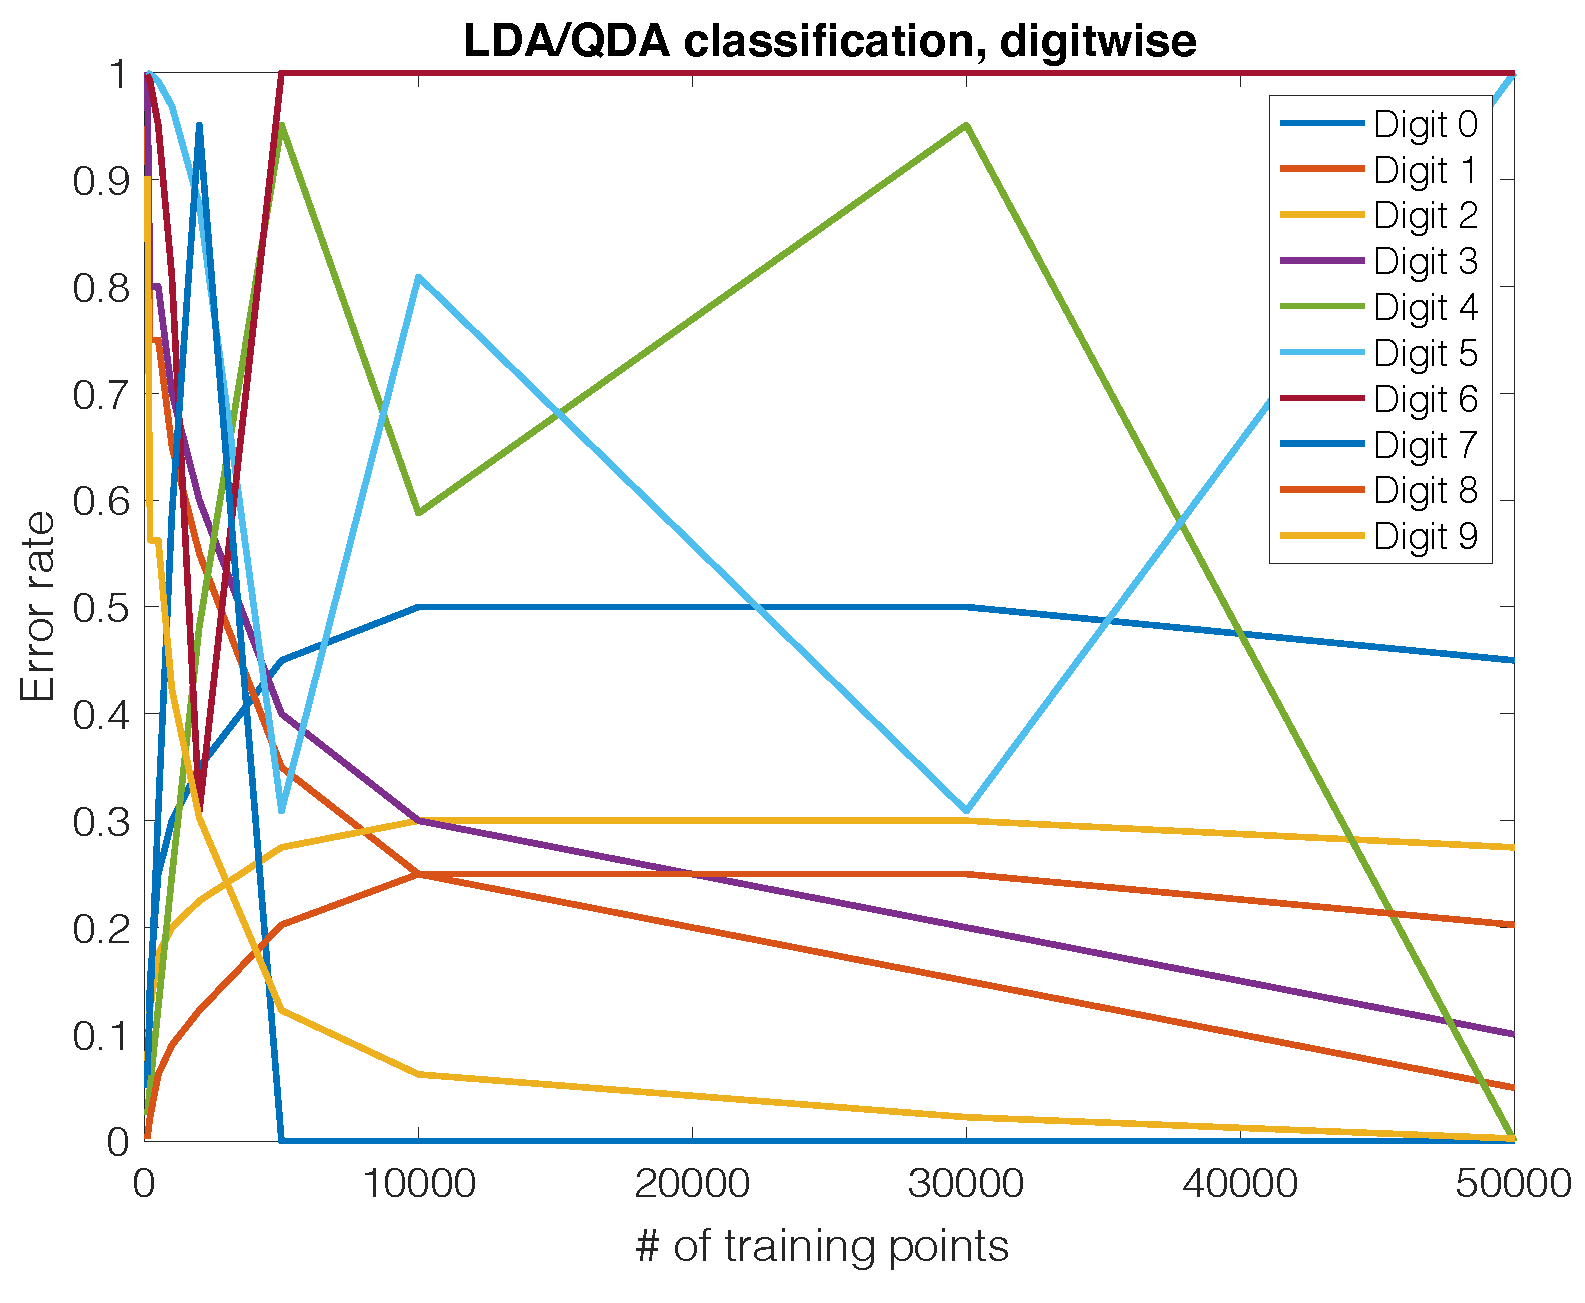
\includegraphics[width=100mm]{HWfig73d.png}
\caption{ \label{fig:epsart} Sample graph with 10 plots}
\end{figure}

\end{enumerate}

\begin{solution}
Your 8.2 solution here. Remember to include graphs and written answers where appropriate 
\end{solution}

\item Using the {\tt mnist\_data.mat}, train your best classifier for the {\tt training\_data} and classify the images in the {\tt test\_data}.  Submit your labels to the online Kaggle competition.  Record your optimum prediction rate in your submission.  You are welcome to compute extra features for the Kaggle competition, as long as they do not use an exterior learned model for their computation (no transer learning!).  If you do so, please describe your implementation in your assignment.
  Please use extra features {\bf only} for the Kaggle portion of the assignment.

\begin{solution}
\textbf{Kaggle Username:} Fill in your kaggle username here!\\
\textbf{Kaggle Score:} Fill in your kaggle score here\\
Answer the written question here 
\end{solution}

\item Next, apply LDA or QDA (your choice) to spam. Submit your test results to the online Kaggle competition. Record your optimum prediction rate in your submission.  If you use additional features (or omit features), please describe them.

\emph{Optional:}  If you use the defaults, expect relatively low classification rates.  We suggest using a Bag-Of-Words model. You are encouraged to explore alternative hand-crafted features, and are welcome to use any third-party library to implement them, as long as they do not use a separate model for their computation (no word-2-vec!).

\begin{solution}
\textbf{Kaggle Username:} Fill in your kaggle username here!\\
\textbf{Kaggle Score:} Fill in your kaggle score here\\
Answer the written question here 
\end{solution}

\end{enumerate}
\pagebreak
\section*{Submission Checklist}
Please ensure you have completed the following before your final submission.
\subsection*{At the beginning of your writeup...}
\begin{enumerate}
    \item Have you copied and hand-signed the honor code specified in Question 1?
    \item Have you listed all students (Names and ID numbers) that you collaborated with?
\end{enumerate}
\subsection*{In your writeup for Question 8...}
\begin{enumerate}
\item Have you included your \textbf{Kaggle Score} and \textbf{Kaggle Username} for \textbf{both} questions 8.4 and 8.5?


\end{enumerate}
\subsection*{At the end of the writeup...}
\begin{enumerate}

\item Have you provided a code appendix including all code you wrote in solving the homework?
\item Have you included featurize.py in your code appendix if you modified it?
\end{enumerate}
\subsection*{Executable Code Submission}
\begin{enumerate}
    \item Have you created an archive containing all ".py" files that you wrote or modified to generate your homework solutions (including featurize.py if you modified it)?
    \item Have you removed all data and extraneous files from the archive?
    \item Have you included a Readme.md in your archive containing any special instructions to reproduce your results?
\end{enumerate}
\subsection*{Submissions}
\begin{enumerate}
    \item Have you submitted your written solutions to the Gradescope assignment titled \textbf{HW3 Write-Up} and selected pages appropriately?
    \item Have you submitted your executable code archive to the Gradescope assignment titled \textbf{HW3 Code}?
    \item Have you submitted your test set predictions for both \textbf{MNIST} and \textbf{SPAM} to the appropriate Kaggle challenges?
\end{enumerate}
Congratulations! You have completed Homework 3.

\end{document}
